\documentclass[spec, och, otchet, hidelinks]{SCWorks}
% параметр - тип обучения - одно из значений:
%    spec     - специальность
%    bachelor - бакалавриат (по умолчанию)
%    master   - магистратура
% параметр - форма обучения - одно из значений:
%    och   - очное (по умолчанию)
%    zaoch - заочное
% параметр - тип работы - одно из значений:
%    otchet
%    referat    - реферат
%    coursework - курсовая работа (по умолчанию)
%    diploma    - дипломная работа
%    pract      - отчет по практике
%    pract      - отчет о научно-исследовательской работе
%    autoref    - автореферат выпускной работы
%    assignment - задание на выпускную квалификационную работу
%    review     - отзыв руководителя
%    critique   - рецензия на выпускную работу
% параметр - включение шрифта
%    times    - включение шрифта Times New Roman (если установлен)
%               по умолчанию выключен
\usepackage[T2A]{fontenc}
\usepackage[utf8]{inputenc}
\usepackage{graphicx}

\usepackage[sort,compress]{cite}
\usepackage{amsmath}
\usepackage{amssymb}
\usepackage{amsthm}
\usepackage{fancyvrb}
\usepackage{longtable}
\usepackage{array}
\usepackage[english,russian]{babel}
\usepackage{minted}
% Используется автором репозитория
%\usemintedstyle{xcode}
% Этот пакет включает в себя аналогичный Times New Roman шрифт.
% Необходим для успешной компиляции для UNIX-систем ввиду отсутствия TNR в нем.
% Можно использовать и для Windows.
\usepackage{tempora}


\usepackage[colorlinks=false]{hyperref}

\graphicspath{{figures/}}

\newcommand{\eqdef}{\stackrel {\rm def}{=}}

\usepackage{stackengine}
\newcommand\xrowht[2][0]{\addstackgap[.5\dimexpr#2\relax]{\vphantom{#1}}}

\newtheorem{lem}{Лемма}

% % При использовании biblatex вместо bibtex
%\usepackage[style=gost-numeric]{biblatex}
%\addbibresource{thesis.bib}

\begin{document}

% Кафедра (в родительном падеже)
\chair{математической кибернетики и компьютерных наук}

% Тема работы
\title{Преобразователи кодов}

% Курс
\course{3}

% Группа
\group{331}

% Факультет (в родительном падеже) (по умолчанию "факультета КНиИТ")
%\department{факультета КНиИТ}

% Специальность/направление код - наименование
%\napravlenie{02.03.02 "--- Фундаментальная информатика и информационные технологии}
%\napravlenie{02.03.01 "--- Математическое обеспечение и администрирование информационных систем}
%\napravlenie{09.03.01 "--- Информатика и вычислительная техника}
%\napravlenie{09.03.04 "--- Программная инженерия}
\napravlenie{10.05.01 "--- Компьютерная безопасность}

% Для студентки. Для работы студента следующая команда не нужна.
%\studenttitle{Студентки}

% Фамилия, имя, отчество в родительном падеже
\author{Бородина Артёма Горовича}

% Заведующий кафедрой
\chtitle{доцент, к.\,ф.-м.\,н.} % степень, звание
\chname{С.\,В.\,Миронов}

%Научный руководитель (для реферата преподаватель проверяющий работу)
\satitle{аспирант}%, к.\,ф.-м.\,н.} %должность, степень, звание
\saname{А.\,А.\,Мартышкин}

% Руководитель практики от организации (только для практики,
% для остальных типов работ не используется)
\patitle{к.\,ф.-м.\,н., доцент}
\paname{Д.\,Ю.\,Петров}

% Семестр (только для практики, для остальных
% типов работ не используется)
\term{2}

% Наименование практики (только для практики, для остальных
% типов работ не используется)
\practtype{учебная}

% Продолжительность практики (количество недель) (только для практики,
% для остальных типов работ не используется)
\duration{2}

% Даты начала и окончания практики (только для практики, для остальных
% типов работ не используется)
\practStart{01.07.2016}
\practFinish{14.07.2016}

% Год выполнения отчета
\date{2022}

\maketitle

% Включение нумерации рисунков, формул и таблиц по разделам
% (по умолчанию - нумерация сквозная)
% (допускается оба вида нумерации)
%\secNumbering


\tableofcontents

% Раздел "Обозначения и сокращения". Может отсутствовать в работе
% \abbreviations
% \begin{description}
%     \item ... "--- ...
%     \item ... "--- ...
% \end{description}

% Раздел "Определения". Может отсутствовать в работе
%\definitions

% Раздел "Определения, обозначения и сокращения". Может отсутствовать в работе.
% Если присутствует, то заменяет собой разделы "Обозначения и сокращения" и "Определения"
%\defabbr


% Раздел "Введение"

\intro

\par Целью данной работы служит ознакомление с устройством и функционированием регистров и регистровой памяти, а также испытание интегрального 
универсального регистра сдвига.

\newpage

\section*{Задание 1.}
\addcontentsline{toc}{section}{Задание 1}

Запустить лабораторный комплекс Labworks и среду МS10. Открыть файл \textbf{33.4.ms10}, размещенный в папке \textbf{Circuit Design Suitе 10.0} среды 
МS10, или собрать на рабочем поле среды MS10 схему для испытания \textit{универсального регистра сдвига} и установить в диалоговых окнах компонентов их 
параметры или режимы работы. \textbf{Скопировать} схему в отчет.

\begin{figure}[h]
	\center{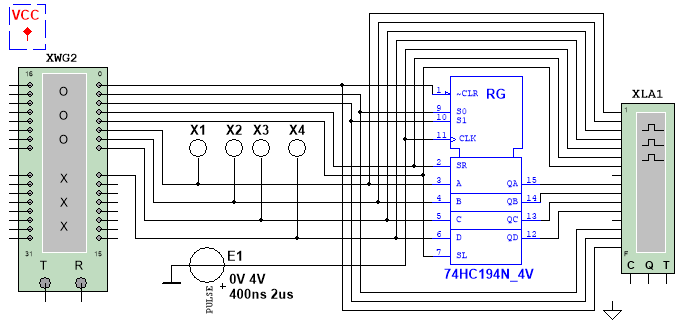
\includegraphics[scale=0.9]{scheme.png}}
	\caption{Схема универсального регистра сдвига.}
\end{figure}

\newpage

\section*{Задание 2.}
\addcontentsline{toc}{section}{Задание 2}

\textbf{Составить} план исследования параллельного регистра сдвига, заполнив ячейки памяти генератора слова \textbf{XWG1} на основе правил 
функционирования регистра \textbf{74НС194\_4V}, отраженных в табл. 1.

\begin{figure}[h]
	\center{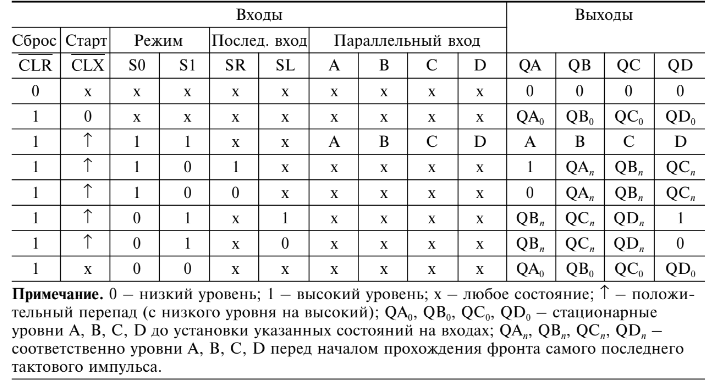
\includegraphics[scale=0.7]{table.png}}
	\caption{Основы правил функционирования регистра \textbf{74НС194\_4V}.}
\end{figure}

\textbf{Запустить} программу моделирования параллельного регистра, \textbf{скопировать} в  отчет программу и временные диаграммы сигналов на входах 
и выходах регистра.

\begin{figure}[h]
	\center{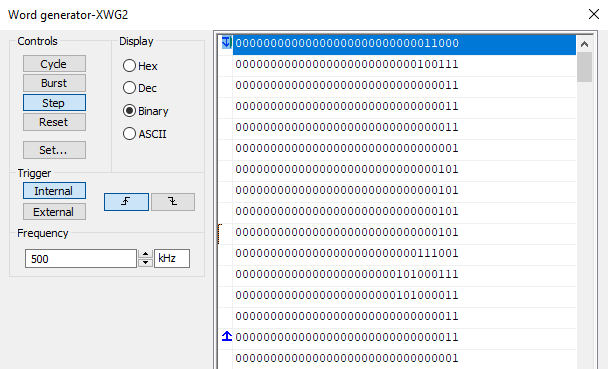
\includegraphics[scale=0.77]{word_generator_task_two.png}}
	\caption{Ячейка памяти генератора слов \textbf{XWG1}.}
\end{figure}

\newpage

\begin{figure}[h!]
	\center{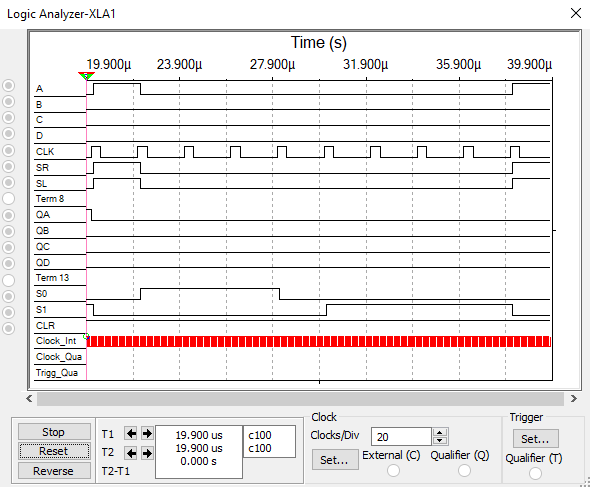
\includegraphics[scale=0.82]{logic_analyzer_task_two_first.png}}
    \caption{Временные диаграммы сигналов на входах и выходах первой части последовательности.}
\end{figure}

\begin{figure}[h!]
	\center{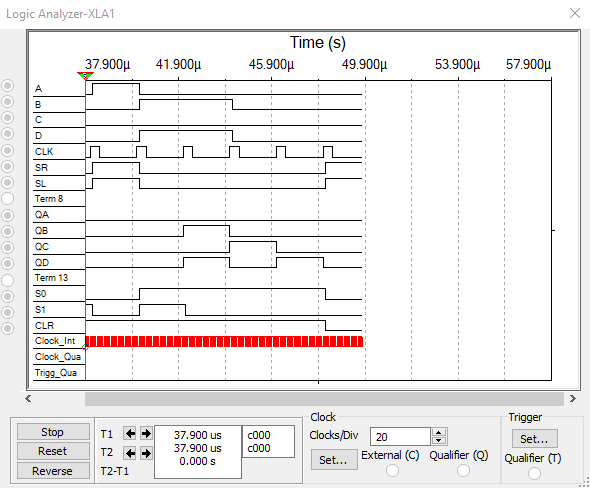
\includegraphics[scale=0.82]{logic_analyzer_task_two_second.png}}
	\caption{Временные диаграммы сигналов на входах и выходах второй части последовательности.}
\end{figure}

\newpage

\section*{Задание 3.}
\addcontentsline{toc}{section}{Задание 3}

Открыть файл \textbf{33.7.ms10}, размещенный в папке \textbf{Circuit Design Suitе 10.0} среды МS10, или собрать на рабочем поле среды MS10 схему для 
испытания \textit{последовательного регистра сдвига} и установить в диалоговых окнах компонентов их параметры или режимы работы. \textbf{Скопировать} 
схему в отчет.

\begin{figure}[h]
	\center{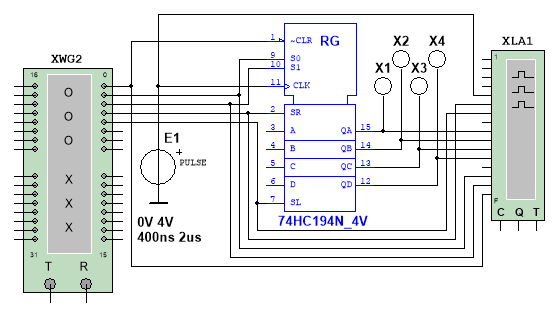
\includegraphics{scheme_task_three.png}}
	\caption{Схема последовательного регистра сдвига.}
\end{figure}

\newpage

\section*{Задание 4.}
\addcontentsline{toc}{section}{Задание 4}

\textbf{Составить} план исследования последовательного регистра \textbf{74НС194\_4V}, заполнив ячейки памяти генератора \textbf{XWG1} произвольными 4-разрядными кодовыми комбинациями, вводимыми последовательно в регистр А.

\begin{figure}[h]
	\center{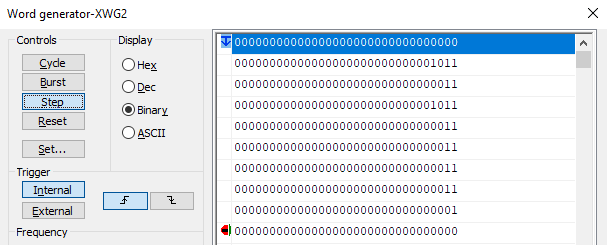
\includegraphics{word_generator_sequences_task_three.png}}
	\caption{Ячейки памяти генератора \textbf{XWG1}.}
\end{figure}

\par \textbf{Запустить} программу моделирования последовательного регистра, \textbf{скопировать} в отчет временные диаграммы сигналов на входах и выходах 
регистра при сдвиге данных влево и вправо.

\begin{figure}[h]
	\center{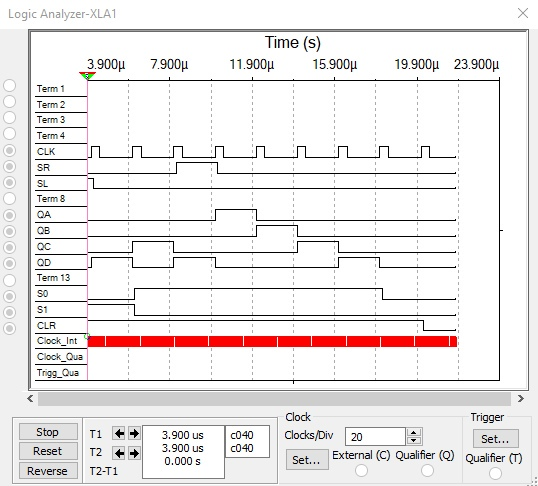
\includegraphics[scale=0.6]{logic_analyzer_task_three.png}}
	\caption{Временные диаграммы сигналов на входах и выходах регистра при сдвиге данных.}
\end{figure}

\newpage

\section*{Тестовые задания}
\addcontentsline{toc}{section}{Тестовые задания}

\par 1. Укажите \textbf{функции}, которые в общем случае может выполнять регистр: 1) \textbf{обнуление (очистку) хранимой информации, запись входной 
	информации в последовательном или в параллельном коде}, 2) \textbf{преобразование информации путём её сдвига под воздействием тактовых импульсов}, 
3) \textbf{Хранение информации, её сдвиг вправо и влево, выдачу хранимой информации в последовательном или в параллельном коде};
\par 2. В параллельном регистре с приходом каждого тактового импульса информация на выходах поразрядно сдвигается в направлении от выхода \textbf{QD} 
к выходу \textbf{QА}. Укажите, как \textbf{называют} такой регистр: \textbf{регистр прямого сдвига};

\par 3. Укажите, какие регистры выполняют со \textbf{статическим} управлением: \textbf{последовательные};

\par 4. Укажите, при каких \textbf{уровнях сигналов} на управляющих входах \textbf{S0} и \textbf{S1} информационные входы реверсивного регистра 
\textbf{74НС194\_4V} недоступны: \textbf{S0 = 0, S1 = 0};

\par 5. Укажите, в какой \textbf{разряд} вводится информация последовательного регистра \textbf{74НС194\_4V} при \textbf{S0} = 1, \textbf{S1} = 0 на 
управляющих входах и сигналах \textbf{SR} = 1 и $ \overline{CLR} = 1 $: \textbf{в рязряд A};

\par 6. Укажите, при \textbf{каких уровнях} управляющих сигналов \textbf{S0} и \textbf{S1} разрешена запись информации в параллельный регистр 
\textbf{74НС194\_4V}: \textbf{S0 = 1, S1 = 1};

\par 7. Укажите, разрешено ли последовательное \textbf{перемещение} сигналов в триггерной подсистеме параллельного регистра \textbf{74НС194\_4V} во 
время записи информации: \textbf{нет};

\par 8. Укажите, сколько \textbf{входов} имеет последовательный регистр с динамическим управлением: \textbf{три: один информационный, вход для тактовых импульсов и установочный вход};

\par 9. Укажите, чем отличается \textbf{динамическое управление} регистрами от статического
управления: \textbf{при динамическом управлении запоминание сигналов, действующих на информационных входах регистра, происходит во входных емкостях \textbf{МДП}-
транзисторов в момент изменения значения сигнала на входе синхронизации, а в статических регистрах, построенных, например, на \textit{RS}-триггерах, 
сигналы действуют в момент их поступления на информационные входы.}

\newpage

\conclusion

\par В ходе лабораторной работы мы ознакомились с устройством и функционированием регистров и регистровой памяти, а также испытали интегральный 
универсальный регистр сдвига на практике. 

\end{document}